\begin{minipage}{.3\textwidth}
    \raggedright
    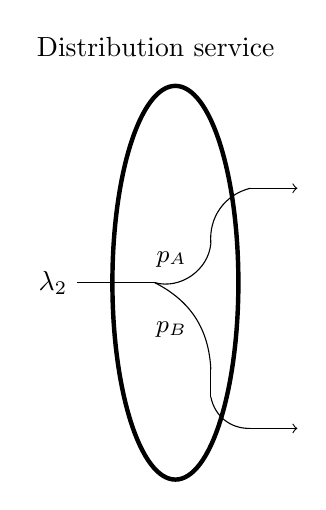
\begin{tikzpicture}
        \draw[ultra thick] (0.75,2) ellipse (0.8cm and 2.5cm);
        \node at (0.5, 5) {Distribution service};
        \draw[-] (0.5, 2) -- ++(-1, 0) node[left] {\(\lambda_2\)};

        % p_A line
        \path (0.49, 2) edge [bend right=50] (1.2, 2.5);
        \path (1.2, 2.5) edge [bend left=40] (1.7, 3.2);
        \draw[->] (1.7, 3.2) -- ++(0.6, 0.);

        % p_B line
        \path (0.49, 2) edge [bend left=30] (1.2, 0.9);
        \draw[-] (1.2, 0.9) -- (1.2, 0.55);
        \path (1.2, 0.55) edge [bend right=40] (1.7, 0.15);
        \draw[->] (1.7, 0.15) -- ++(0.6, 0.);

        \node at (0.7, 2.3) {\small{\( p_A \)}};
        \node at (0.7, 1.4) {\small{\( p_B \)}};
    \end{tikzpicture}
\end{minipage}
\begin{minipage}{.65\textwidth}
    \centering
    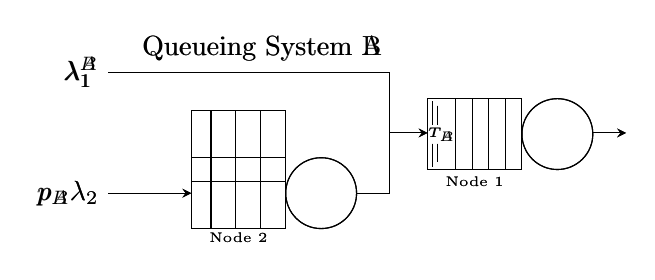
\begin{tikzpicture}[>=stealth, scale=0.6] %arrow type
        % Difference between the two queue diagrams
        
        \tikzmath{
            let \diff = -5cm;
        }
            
        % QUEUEING SYSTEM A

        \node at (1.5cm, 2.3cm) {Queueing System A};
            
        % the rectangle with vertical lines (Node 2)
        \draw (0,0) -- ++(2cm,0) -- ++(0,-1.5cm) -- ++(-2cm,0);
        \foreach \i in {1,...,3, 3.8}
        \draw (2cm-\i*15pt,0) -- +(0,-1.5cm);
        \node at (1, -1.7) {\tiny{Node 2}};

        % the circle (Node 2)
        \draw (2.75,-0.75cm) circle [radius=0.75cm];

        % the rectangle with vertical lines (Node 1)
        \draw (5,1.25) -- ++(2cm,0) -- ++(0,-1.5cm) -- ++(-2cm,0);
        \foreach \i in {1,...,4, 5.7}
        \draw (7cm-\i*10pt,1.25) -- +(0,-1.5cm);
        \node at (6, -0.5) {\tiny{Node 1}};

        % The two vertical lines at the start of Node 1
        \draw (7cm-54pt, 1.2cm) -- +(0,-0.5cm);
        \draw (7cm-54pt, 0.3cm) -- +(0,-0.5cm);
        \draw (7cm-51pt, 1.1cm) -- +(0,-0.4cm);
        \draw (7cm-51pt, 0.3cm) -- +(0,-0.4cm);

        % The label between the lines for T
        \node[anchor=north] at (5.3, 0.84) {\tiny{\( T_A \)}};

        % the circle (Node 1)
        \draw (7.75,0.5) circle [radius=0.75cm];

        % the arrows and labels (Node 2+2)
        \draw[->] (8.5,0.525) -- +(20pt,0);

        % Ambulance lines
        \draw[<-] (0,-0.75) -- +(-50pt,0) node[left] {\( p_A \lambda_2 \)};
        \draw[-] (3.5,-0.75) -- +(20pt,0);
        \draw (4.2, 0.525) -- (4.2, -0.75);

        % Others lines
        \draw (4.2, 1.8) -- +(-169.5pt,0) node[left] {\( \lambda_1^A \)};
        \draw (4.2, 1.8) -- (4.2, 0.525);
        \draw[->] (4.2, 0.525) -- (5, 0.525);


        % QUEUEING SYSTEM B

        \node at (1.5cm, \diff + 2.3cm) {Queueing System B};

        % the rectangle with vertical rules (Node 2)
        \draw (0, \diff) -- ++(2cm,0) -- ++(0,-1.5cm) -- ++(-2cm,0);
        \foreach \i in {1,...,3, 3.8}
        \draw (2cm-\i*15pt,\diff) -- +(0,-1.5cm);
        \node at (1cm, \diff - 1.7cm) {\tiny{Node 2}};

        % the circle (Node 2)
        \draw (2.75,\diff - 0.75cm) circle [radius=0.75cm];

        % the rectangle with vertical rules (Queue 2)
        \draw (5,\diff + 1.25cm) -- ++(2cm,0) -- ++(0,-1.5cm) -- ++(-2cm,0);
        \foreach \i in {1,...,4, 5.7}
        \draw (7cm-\i*10pt,\diff + 1.25cm) -- +(0,-1.5cm);
        \node at (6, \diff - 0.5cm) {\tiny{Node 1}};

        % The two vertical lines at the start of Queue 2
        \draw (7cm-54pt,\diff + 1.2cm) -- +(0,-0.5cm);
        \draw (7cm-54pt,\diff + 0.3cm) -- +(0,-0.5cm);
        \draw (7cm-51pt,\diff + 1.1cm) -- +(0,-0.4cm);
        \draw (7cm-51pt,\diff + 0.3cm) -- +(0,-0.4cm);

        % The label between the lines for T
        \node[anchor=north] at (5.3, \diff + 0.84cm) {\tiny{\( T_B \)}};

        % the circle (Queue 2)
        \draw (7.75,\diff + 0.5cm) circle [radius=0.75cm];

        % the arrows and labels (Node 2+2)
        \draw[->] (8.5, \diff + 0.525cm) -- +(20pt,0);

        % Ambulance lines
        \draw[<-] (0, \diff - 0.75cm) -- +(-50pt,0) node[left]
        {\( p_B \lambda_2 \)};
        \draw[-] (3.5, \diff - 0.75cm) -- +(20pt,0);
        \draw (4.2, \diff + 0.525cm) -- (4.2, \diff - 0.75cm);

        % Others lines
        \draw (4.2, \diff + 1.8cm) -- +(-169.5pt,0) node[left]
        {\( \lambda_1^B \)};
        \draw (4.2, \diff + 1.8cm) -- (4.2, \diff + 0.525);
        \draw[->] (4.2, \diff + 0.525cm) -- (5, \diff + 0.525cm);
    \end{tikzpicture}
\end{minipage}
